% Options for packages loaded elsewhere
\PassOptionsToPackage{unicode}{hyperref}
\PassOptionsToPackage{hyphens}{url}
%
\documentclass[
  ignorenonframetext,
  aspectratio=169]{beamer}
\usepackage{pgfpages}
\setbeamertemplate{caption}[numbered]
\setbeamertemplate{caption label separator}{: }
\setbeamercolor{caption name}{fg=normal text.fg}
\beamertemplatenavigationsymbolsempty
% Prevent slide breaks in the middle of a paragraph
\widowpenalties 1 10000
\raggedbottom
\setbeamertemplate{part page}{
  \centering
  \begin{beamercolorbox}[sep=16pt,center]{part title}
    \usebeamerfont{part title}\insertpart\par
  \end{beamercolorbox}
}
\setbeamertemplate{section page}{
  \centering
  \begin{beamercolorbox}[sep=12pt,center]{part title}
    \usebeamerfont{section title}\insertsection\par
  \end{beamercolorbox}
}
\setbeamertemplate{subsection page}{
  \centering
  \begin{beamercolorbox}[sep=8pt,center]{part title}
    \usebeamerfont{subsection title}\insertsubsection\par
  \end{beamercolorbox}
}
\AtBeginPart{
  \frame{\partpage}
}
\AtBeginSection{
  \ifbibliography
  \else
    \frame{\sectionpage}
  \fi
}
\AtBeginSubsection{
  \frame{\subsectionpage}
}
\usepackage{amsmath,amssymb}
\usepackage{lmodern}
\usepackage{ifxetex,ifluatex}
\ifnum 0\ifxetex 1\fi\ifluatex 1\fi=0 % if pdftex
  \usepackage[T1]{fontenc}
  \usepackage[utf8]{inputenc}
  \usepackage{textcomp} % provide euro and other symbols
\else % if luatex or xetex
  \usepackage{unicode-math}
  \defaultfontfeatures{Scale=MatchLowercase}
  \defaultfontfeatures[\rmfamily]{Ligatures=TeX,Scale=1}
\fi
\usetheme[]{metropolis}
% Use upquote if available, for straight quotes in verbatim environments
\IfFileExists{upquote.sty}{\usepackage{upquote}}{}
\IfFileExists{microtype.sty}{% use microtype if available
  \usepackage[]{microtype}
  \UseMicrotypeSet[protrusion]{basicmath} % disable protrusion for tt fonts
}{}
\makeatletter
\@ifundefined{KOMAClassName}{% if non-KOMA class
  \IfFileExists{parskip.sty}{%
    \usepackage{parskip}
  }{% else
    \setlength{\parindent}{0pt}
    \setlength{\parskip}{6pt plus 2pt minus 1pt}}
}{% if KOMA class
  \KOMAoptions{parskip=half}}
\makeatother
\usepackage{xcolor}
\IfFileExists{xurl.sty}{\usepackage{xurl}}{} % add URL line breaks if available
\IfFileExists{bookmark.sty}{\usepackage{bookmark}}{\usepackage{hyperref}}
\hypersetup{
  pdfauthor={Olivier Gimenez},
  hidelinks,
  pdfcreator={LaTeX via pandoc}}
\urlstyle{same} % disable monospaced font for URLs
\newif\ifbibliography
\usepackage{graphicx}
\makeatletter
\def\maxwidth{\ifdim\Gin@nat@width>\linewidth\linewidth\else\Gin@nat@width\fi}
\def\maxheight{\ifdim\Gin@nat@height>\textheight\textheight\else\Gin@nat@height\fi}
\makeatother
% Scale images if necessary, so that they will not overflow the page
% margins by default, and it is still possible to overwrite the defaults
% using explicit options in \includegraphics[width, height, ...]{}
\setkeys{Gin}{width=\maxwidth,height=\maxheight,keepaspectratio}
% Set default figure placement to htbp
\makeatletter
\def\fps@figure{htbp}
\makeatother
\setlength{\emergencystretch}{3em} % prevent overfull lines
\providecommand{\tightlist}{%
  \setlength{\itemsep}{0pt}\setlength{\parskip}{0pt}}
\setcounter{secnumdepth}{-\maxdimen} % remove section numbering
% Allowing for slides with 2 columns
\def\begincols{\begin{columns}[c]}
\def\endcols{\end{columns}}
\def\begincol{\begin{column}{0.5\textwidth}}
\def\endcol{\end{column}}

% Reducing black space between R code and output
% \setlength{\topsep}{0pt}{}
\setlength{\emergencystretch}{0em}
\setlength{\parskip}{2pt}
\setlength{\partopsep}{1pt}

% Reducing font size of R code and output
% Code below from http://stackoverflow.com/a/38324868
% See also http://stackoverflow.com/a/39961605

% Change fontsize of R code
\let\oldShaded\Shaded
\let\endoldShaded\endShaded
\renewenvironment{Shaded}{\footnotesize\oldShaded}{\endoldShaded}

% Change fontsize of output
\let\oldverbatim\verbatim
\let\endoldverbatim\endverbatim
\renewenvironment{verbatim}{\footnotesize\oldverbatim}{\endoldverbatim}
\ifluatex
  \usepackage{selnolig}  % disable illegal ligatures
\fi

\title{Bayesian statistics with R\\
1. An introduction to Bayesian inference}
\author{Olivier Gimenez}
\date{November 2021}

\begin{document}
\frame{\titlepage}

\begin{frame}{Credit where credit's due}
\protect\hypertarget{credit-where-credits-due}{}
\begin{itemize}
\item
  Ruth King, Byron Morgan, Steve Brooks (our workshops and
  \href{https://www.maths.ed.ac.uk/~rking33/Book-website/index.html}{\alert{Bayesian analysis for population ecology}
  book}).
\item
  Richard McElreath
  (\href{https://github.com/rmcelreath/statrethinking_winter2019}{\alert{Statistical rethinking}
  book and lecture videos}).
\item
  Jim Albert and Jingchen Hu
  (\href{https://bayesball.github.io/BOOK/probability-a-measurement-of-uncertainty.html}{\alert{Probability and Bayesian modelling}
  book}).
\item
  Materials shared by
  \href{https://www.tjmahr.com/}{\alert{Tristan Marh}},
  \href{https://www.gla.ac.uk/researchinstitutes/bahcm/staff/jasonmatthiopoulos/}{\alert{Jason Matthiopoulos}},
  \href{https://frodriguezsanchez.net/}{\alert{Francisco Rodriguez Sanchez}},
  \href{https://staff.qut.edu.au/staff/k.mengersen}{\alert{Kerrie Mengersen}}
  and \href{https://quantscience.rbind.io/}{\alert{Mark Lai}}.
\end{itemize}
\end{frame}

\begin{frame}[fragile]{Slides, code and data}
\protect\hypertarget{slides-code-and-data}{}
\begin{itemize}
\tightlist
\item
  All material prepared with \texttt{R}.
\item
  \texttt{R\ Markdown} used to write reproducible material.
\item
  Dedicated website
  \href{https://oliviergimenez.github.io/bayesian-stats-with-R/}{\alert{https://oliviergimenez.github.io/bayesian-stats-with-R/}}.
\end{itemize}
\end{frame}

\begin{frame}{Objectives}
\protect\hypertarget{objectives}{}
\begin{itemize}
\tightlist
\item
  Try and demystify Bayesian statistics, and what we call MCMC.
\item
  Make the difference between Bayesian and Frequentist analyses.
\item
  Understand the Methods section of ecological papers doing Bayesian
  stuff.
\item
  Run Bayesian analyses, safely hopefully.
\end{itemize}
\end{frame}

\begin{frame}
\begin{center}
\includegraphics[width=13cm,height=7cm]{img/brace_yourself} \end{center}
\end{frame}

\begin{frame}[fragile]{What is on our plate?}
\protect\hypertarget{what-is-on-our-plate}{}
\begin{enumerate}
\tightlist
\item
  An introduction to Bayesian inference
\item
  The likelihood
\item
  Bayesian analyses by hand
\item
  A detour to explore priors
\item
  Markov chains Monte Carlo methods (MCMC)
\item
  Bayesian analyses in \texttt{R} with the \texttt{Jags} software
\item
  Contrast scientific hypotheses with model selection
\item
  Heterogeneity and multilevel models (aka mixed models)
\end{enumerate}
\end{frame}

\hypertarget{i-want-moooooore}{%
\section{I want moooooore}\label{i-want-moooooore}}

\begin{frame}
\begin{center}
\includegraphics[width=13cm,height=7cm]{img/books} \end{center}
\end{frame}

\begin{frame}
\begin{center}
\includegraphics[width=6.88in]{img/mccarthy} \end{center}
\end{frame}

\begin{frame}
\begin{center}
\includegraphics[width=8.58in]{img/kery} \end{center}
\end{frame}

\begin{frame}
\begin{center}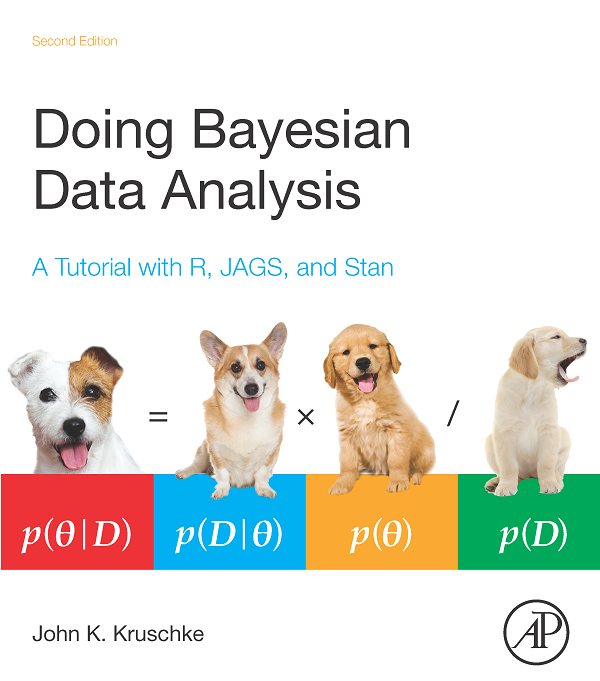
\includegraphics[width=8.33in]{img/kruschke} \end{center}
\end{frame}

\begin{frame}
\begin{center}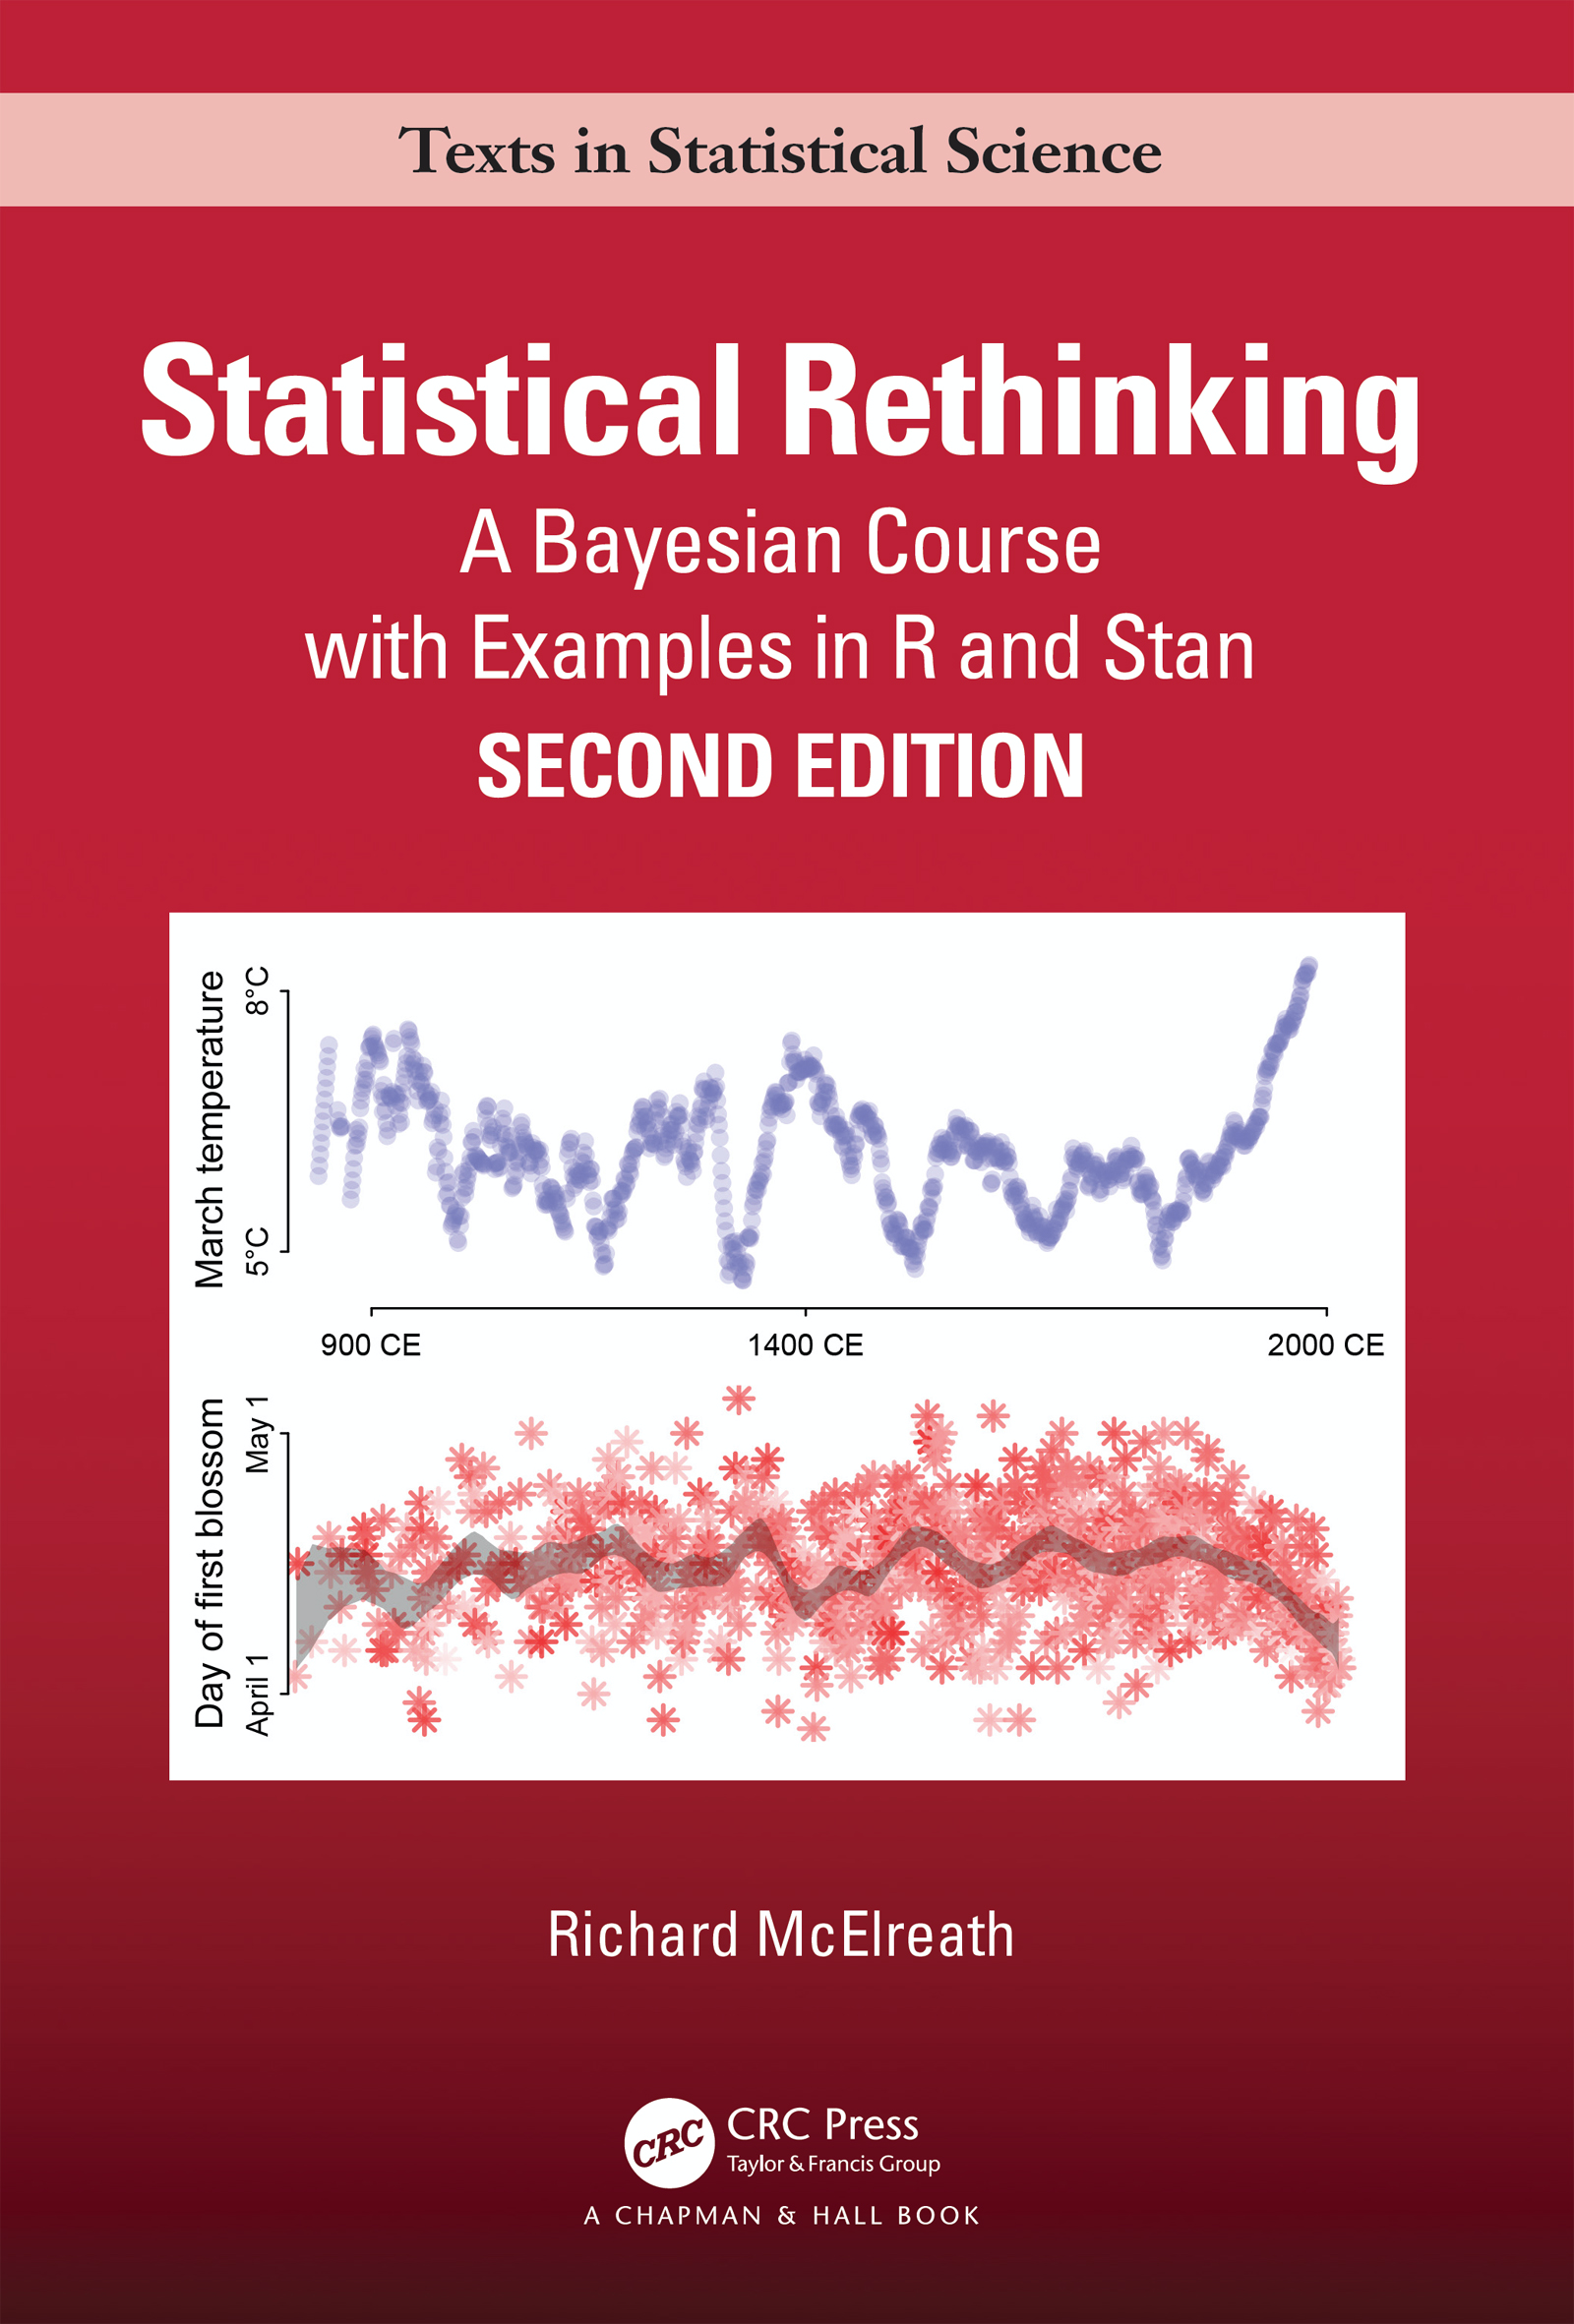
\includegraphics[width=22.22in]{img/mcelreath} \end{center}
\end{frame}

\begin{frame}
\begin{center}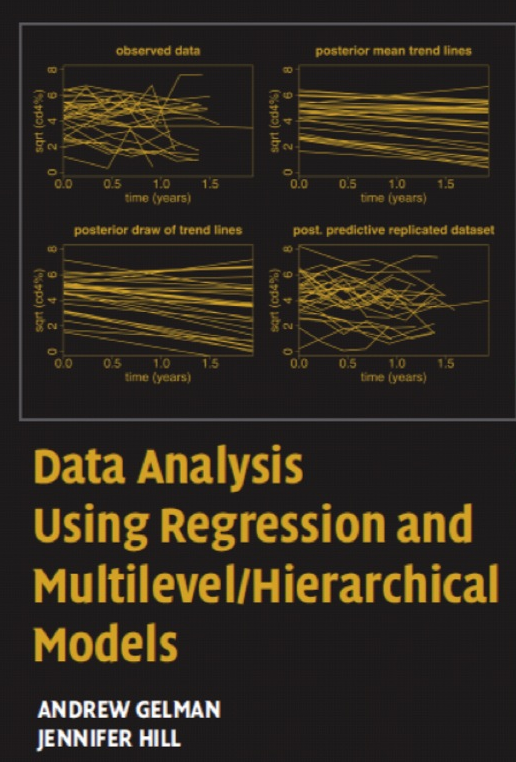
\includegraphics[width=7.17in]{img/gelmanhill} \end{center}
\end{frame}

\begin{frame}
\begin{center}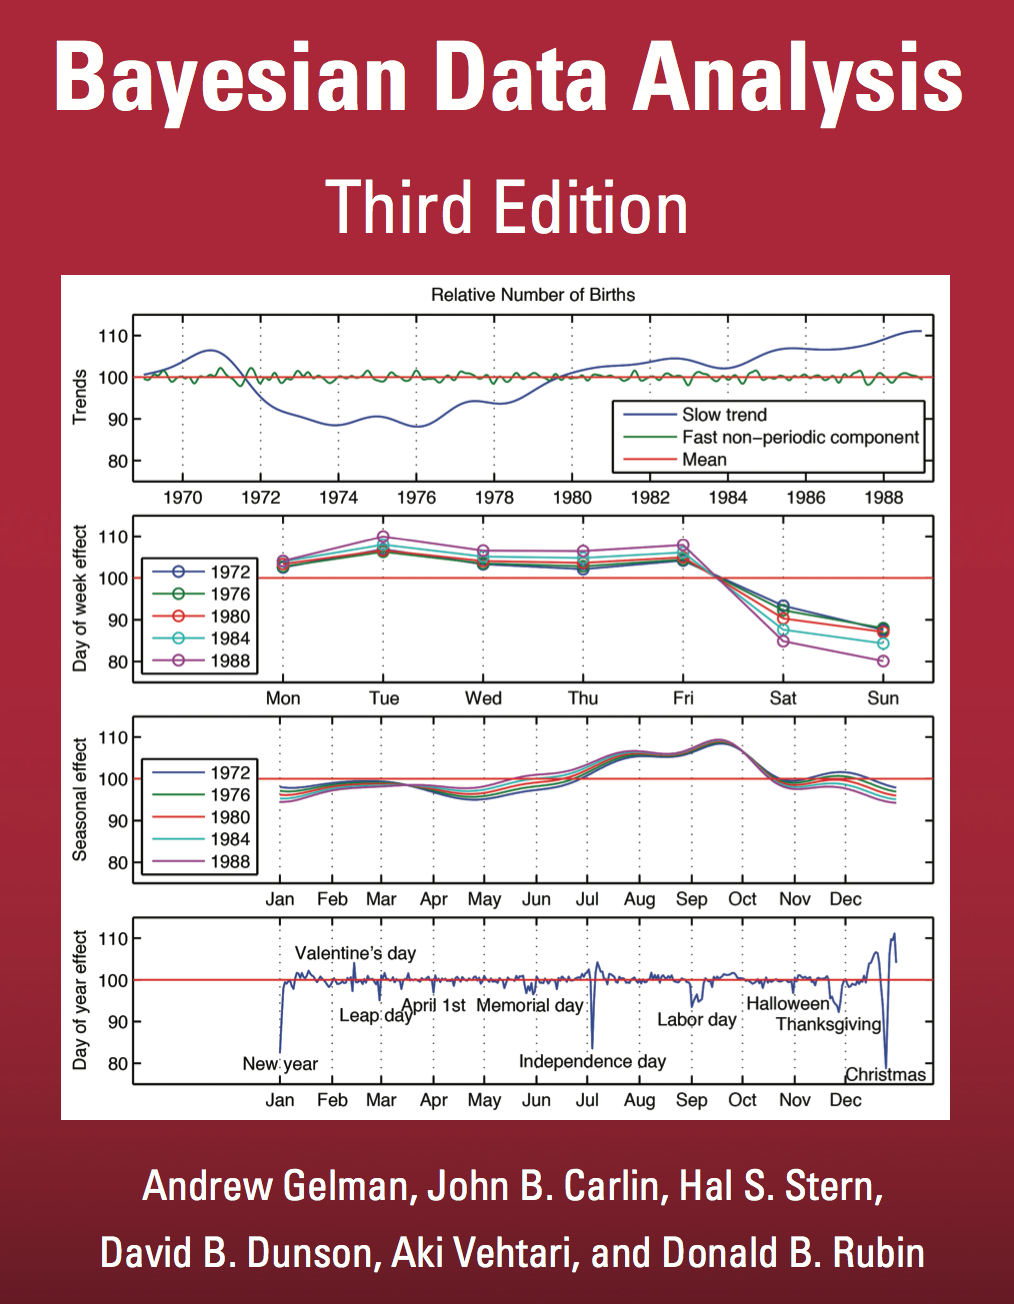
\includegraphics[width=13cm,height=7cm]{img/bda_cover} \end{center}

Free at \url{http://www.stat.columbia.edu/~gelman/book/}
\end{frame}

\hypertarget{what-is-bayesian-inference}{%
\section{What is Bayesian inference?}\label{what-is-bayesian-inference}}

\begin{frame}

\includegraphics{img/amazing-thomas-bayes-illustration.jpg}
\end{frame}

\begin{frame}{A reminder on conditional probabilities}
\protect\hypertarget{a-reminder-on-conditional-probabilities}{}
\begin{itemize}[<+->]
\tightlist
\item
  \(\Pr(A \mid B)\): Probability of A given B
\end{itemize}

\begin{itemize}[<+->]
\tightlist
\item
  The ordering matters: \(\Pr(A \mid B)\) is not the same as
  \(\Pr(B \mid A)\).
\end{itemize}

\begin{itemize}[<+->]
\tightlist
\item
  \(\Pr(A \mid B) = \displaystyle{\frac{\Pr(A \text{ and } B)}{\Pr(B)}}\)
\end{itemize}
\end{frame}

\begin{frame}

\includegraphics{img/how_to_cure_vampires.jpg}
\end{frame}

\begin{frame}{Screening for vampirism}
\protect\hypertarget{screening-for-vampirism}{}
\begin{itemize}[<+->]
\tightlist
\item
  The chance of the test being positive given you are a vampire is
  \(\Pr(+|\text{vampire}) = 0.90\) (\textbf{sensitivity}).
\end{itemize}

\begin{itemize}[<+->]
\tightlist
\item
  The chance of a negative test given you are mortal is
  \(\Pr(-|\text{mortal}) = 0.95\) (\textbf{specificity}).
\end{itemize}
\end{frame}

\begin{frame}{What is the question?}
\protect\hypertarget{what-is-the-question}{}
\begin{itemize}[<+->]
\tightlist
\item
  From the perspective of the test: Given a person is a vampire, what is
  the probability that the test is positive?
  \(\Pr(+|\text{vampire}) = 0.90\).
\end{itemize}

\begin{itemize}[<+->]
\tightlist
\item
  From the perspective of a person: Given that the test is positive,
  what is the probability that this person is a vampire?
  \(\Pr(\text{vampire}|+) = \; ?\)
\end{itemize}

\begin{itemize}[<+->]
\tightlist
\item
  Assume that vampires are rare, and represent only \(0.1\%\) of the
  population. This means that \(\Pr(\text{vampire}) = 0.001\).
\end{itemize}
\end{frame}

\begin{frame}{What is the answer? Bayes' theorem to the rescue!}
\protect\hypertarget{what-is-the-answer-bayes-theorem-to-the-rescue}{}
\begincols
\begincol

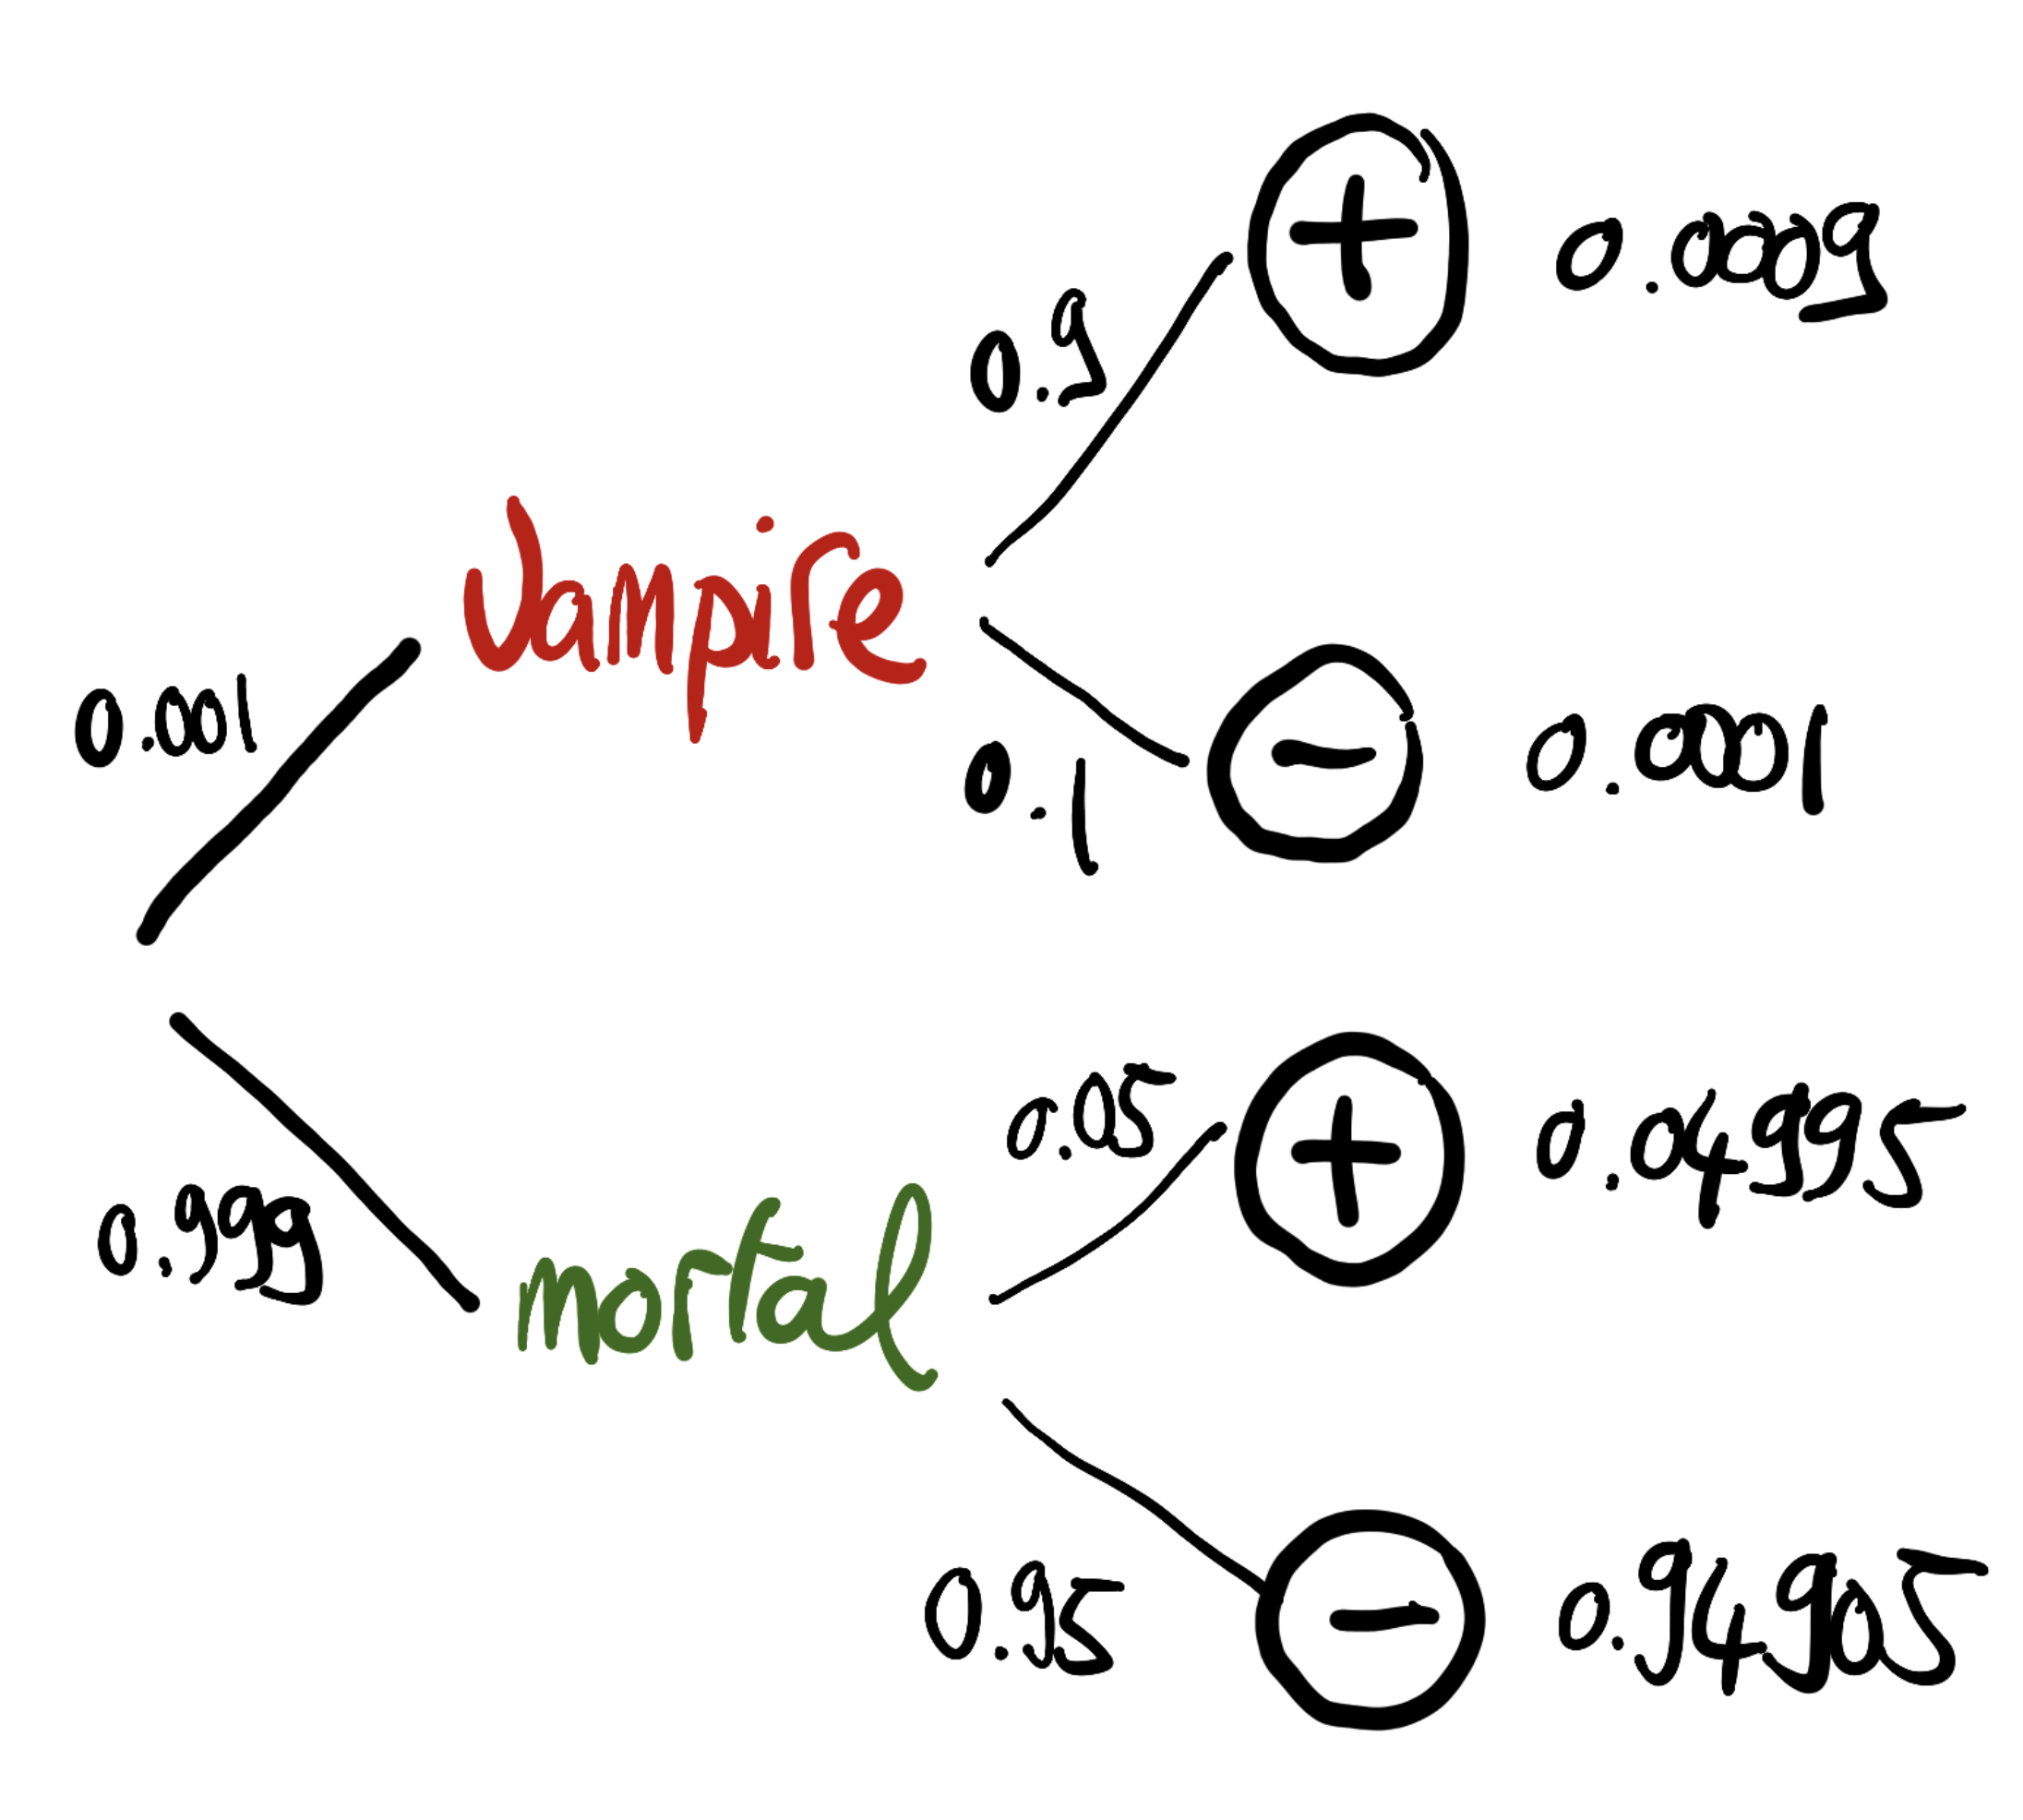
\includegraphics{img/binary_covid.png}

\endcol

\begincol

\begin{itemize}
\tightlist
\item
  \(\Pr(\text{vampire}|+) = \displaystyle{\frac{\Pr(\text{vampire and } +)}{\Pr(+)}}\)
\end{itemize}

\pause

\begin{itemize}
\tightlist
\item
  \(\Pr(\text{vampire and } +) = \Pr(\text{vampire}) \; \Pr(+ | \text{vampire}) = 0.0009\)
\end{itemize}

\pause

\begin{itemize}
\tightlist
\item
  \(\Pr(+) = 0.0009 + 0.04995 = 0.05085\)
\end{itemize}

\pause

\begin{itemize}
\tightlist
\item
  \(\Pr(\text{vampire}|+) = 0.0009/0.05085 = 0.02\)
\end{itemize}

\endcol
\endcols

\pause

\[\Pr(\text{vampire}|+)= \displaystyle{\frac{ \Pr(+|\text{vampire}) \; \Pr(\text{vampire})}{\Pr(+)}}\]
\end{frame}

\hypertarget{your-turn-practical-1}{%
\section{Your turn: Practical 1}\label{your-turn-practical-1}}

\begin{frame}{Bayes' theorem}
\protect\hypertarget{bayes-theorem}{}
\begincols
\begincol

\begin{itemize}
\item
  A theorem about conditional probabilities.
\item
  \(\Pr(B \mid A) = \displaystyle{\frac{ \Pr(A \mid B) \; \Pr(B)}{\Pr(A)}}\)
\end{itemize}

\endcol

\begincol

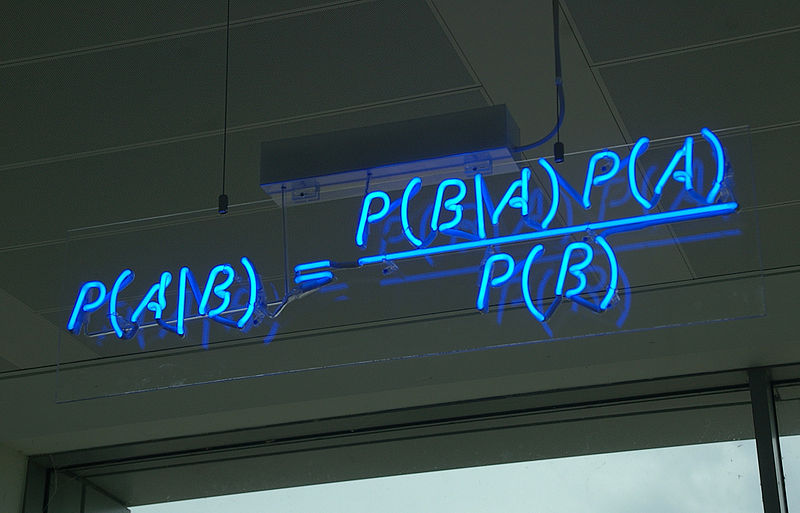
\includegraphics{img/bayes_neon.jpeg}

\endcol
\endcols
\end{frame}

\begin{frame}{Bayes' theorem}
\protect\hypertarget{bayes-theorem-1}{}
\begin{itemize}[<+->]
\tightlist
\item
  Easy to mess up with letters. Might be easier to remember when written
  like this:
\end{itemize}

\[ \Pr(\text{hypothesis} \mid \text{data}) = \frac{ \Pr(\text{data} \mid \text{hypothesis}) \; \Pr(\text{hypothesis})}{\Pr(\text{data})} \]

\begin{itemize}[<+->]
\tightlist
\item
  The ``hypothesis'' is typically something unobserved or unknown. It's
  what you want to learn about using the data.
\end{itemize}

\begin{itemize}[<+->]
\tightlist
\item
  For regression models, the ``hypothesis'' is a parameter (intercept,
  slopes or error terms).
\end{itemize}

\begin{itemize}[<+->]
\tightlist
\item
  Bayes theorem tells you the probability of the hypothesis given the
  data.
\end{itemize}
\end{frame}

\begin{frame}{What is doing science after all?}
\protect\hypertarget{what-is-doing-science-after-all}{}
How plausible is some hypothesis given the data?

\[ \Pr(\text{hypothesis} \mid \text{data}) = \frac{ \Pr(\text{data} \mid \text{hypothesis}) \; \Pr(\text{hypothesis})}{\Pr(\text{data})} \]
\end{frame}

\begin{frame}{Why is Bayesian statistics not the default?}
\protect\hypertarget{why-is-bayesian-statistics-not-the-default}{}
\begin{itemize}[<+->]
\tightlist
\item
  Due to practical problems of implementing the Bayesian approach, and
  some wars of male statisticians's egos, little advance was made for
  over two centuries.
\end{itemize}

\begin{itemize}[<+->]
\tightlist
\item
  Recent advances in computational power coupled with the development of
  new methodology have led to a great increase in the application of
  Bayesian methods within the last two decades.
\end{itemize}
\end{frame}

\begin{frame}{Frequentist versus Bayesian}
\protect\hypertarget{frequentist-versus-bayesian}{}
\begin{itemize}[<+->]
\tightlist
\item
  Typical stats problems involve estimating parameter \(\theta\) with
  available data.
\end{itemize}

\begin{itemize}[<+->]
\tightlist
\item
  The frequentist approach (\textbf{maximum likelihood estimation} --
  MLE) assumes that the parameters are fixed, but have unknown values to
  be estimated.
\end{itemize}

\begin{itemize}[<+->]
\tightlist
\item
  Classical estimates generally provide a point estimate of the
  parameter of interest.
\end{itemize}

\begin{itemize}[<+->]
\tightlist
\item
  The Bayesian approach assumes that the parameters are not fixed but
  have some fixed unknown distribution - a distribution for the
  parameter.
\end{itemize}
\end{frame}

\begin{frame}{What is the Bayesian approach?}
\protect\hypertarget{what-is-the-bayesian-approach}{}
\begin{itemize}
\tightlist
\item
  The approach is based upon the idea that the experimenter begins with
  some prior beliefs about the system.
\end{itemize}

\pause

\begin{itemize}
\tightlist
\item
  And then updates these beliefs on the basis of observed data.
\end{itemize}

\pause

\begin{itemize}
\tightlist
\item
  This updating procedure is based upon the Bayes' Theorem:
\end{itemize}

\[\Pr(A \mid B) = \frac{\Pr(B \mid A) \; \Pr(A)}{\Pr(B)}\]
\end{frame}

\begin{frame}{What is the Bayesian approach?}
\protect\hypertarget{what-is-the-bayesian-approach-1}{}
\begin{itemize}
\tightlist
\item
  Schematically if \(A = \theta\) and \(B = \text{data}\), then
\end{itemize}

\pause

\begin{itemize}
\tightlist
\item
  The Bayes' theorem
\end{itemize}

\[\Pr(A \mid B) = \frac{\Pr(B \mid A) \; \Pr(A)}{\Pr(B)}\]

\pause

\begin{itemize}
\tightlist
\item
  Translates into:
\end{itemize}

\[\Pr(\theta \mid \text{data}) = \frac{\Pr(\text{data} \mid \theta) \; \Pr(\theta)}{\Pr(\text{data})}\]
\end{frame}

\begin{frame}{Bayes' theorem}
\protect\hypertarget{bayes-theorem-2}{}
\[{\color{red}{\Pr(\theta \mid \text{data})}} = \frac{\color{blue}{\Pr(\text{data} \mid \theta)} \; \color{green}{\Pr(\theta)}}{\color{orange}{\Pr(\text{data})}}\]

\pause

\begin{itemize}
\tightlist
\item
  \textcolor{red}{Posterior distribution}: Represents what you know
  after having seen the data. The basis for inference, a distribution,
  possibly multivariate if more than one parameter (\(\theta\)).
\end{itemize}

\pause

\begin{itemize}
\tightlist
\item
  \textcolor{blue}{Likelihood}: We know that quantity, same as in the
  MLE approach.
\end{itemize}

\pause

\begin{itemize}
\tightlist
\item
  \textcolor{green}{Prior distribution}: Represents what you know before
  seeing the data. The source of much discussion about the Bayesian
  approach.
\end{itemize}

\pause

\begin{itemize}
\tightlist
\item
  \(\color{orange}{\Pr(\text{data}) = \int \Pr(\text{data} \mid \theta) \;\Pr(\theta) d\theta }\):
  Possibly high-dimensional integral, difficult if not impossible to
  calculate. This is one of the reasons why we need simulation (MCMC)
  methods - more soon.
\end{itemize}
\end{frame}

\begin{frame}
\begin{center}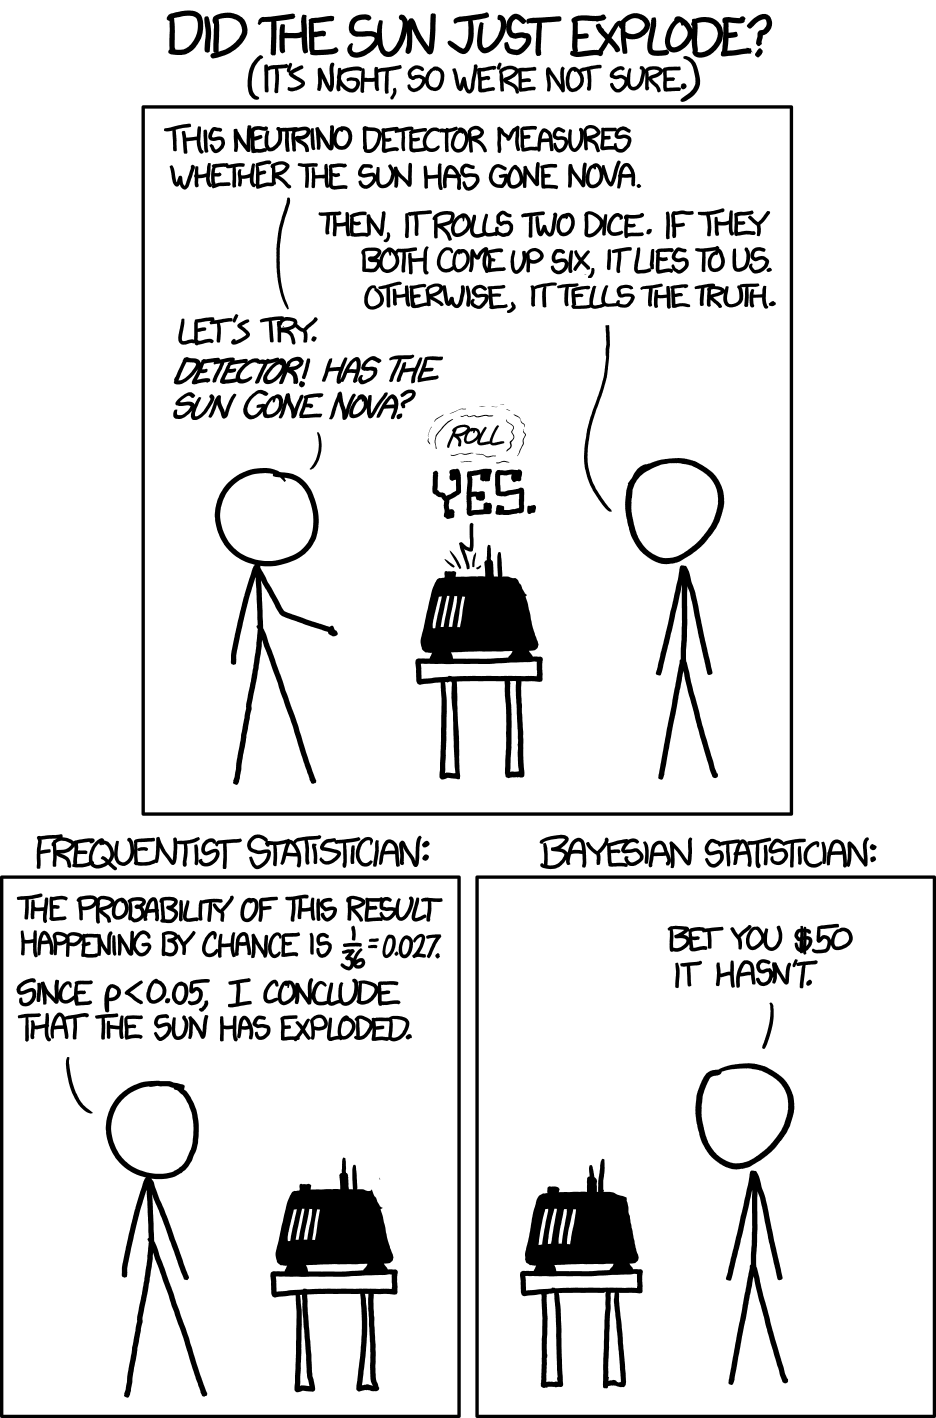
\includegraphics[width=13in]{img/frequentists_vs_bayesians_2x} \end{center}
\end{frame}

\end{document}
